\documentclass[10pt,a4paper,twoside,titlepage,twocolumn]{article}
\usepackage[utf8]{inputenc}
\usepackage[T1]{fontenc}
\usepackage[ngerman]{babel,varioref}
\usepackage[left=0.7cm,right=0.7cm,top=0.7cm,bottom=0.7cm,includeheadfoot]{geometry}
\usepackage{pgfplots}
\pgfplotsset{compat=newest}
\usepackage{amsfonts}
\usepackage{amsmath}
\usepackage{amssymb}
\usepackage{graphicx}
\usepackage{xcolor}
\usepackage{siunitx}
\usepackage{enumitem}
\usepackage{transparent}
\usepackage{cleveref}
\usepackage{fancyhdr}
\pagestyle{fancy}
\newcommand{\rom}[1]{\uppercase\expandafter{\romannumeral #1\relax}}

\begin{document}
\lhead{\textbf{PhyNMS} \\ \textit{Lukas Schöpf}}
\rhead{\date{\today}}
    \graphicspath{ {./Images/} }


\definecolor{formulablue}{RGB}{219,219,255}
\newcommand{\formula}[1]{\colorbox{formulablue}{#1}}

\newcommand{\unitText}[3]{\noindent\textit{#1} : #2 [#3]}

\definecolor{refrot}{RGB}{183,28,42}
\newcommand{\refskript}[1]{\textcolor{refrot}{Skript S.#1}}



% \titlespacing*{\section}{0pt}{12pt}{0pt}
% \titlespacing*{\subsection}{0pt}{0pt}{0pt}
% \titlespacing*{\subsubsection}{0pt}{0pt}{0pt}


\title{\vspace{50mm}MachLe \\ [1ex] \large Summary}
\author{Lukas Schöpf}
% \titlepic{\vspace{50mm}\includegraphics[width=0.25\textwidth]{Elvis}}


% Code format
% Define the Gruvbox light colors
\definecolor{gruvbox_bg}{HTML}{fbf1c7}
\definecolor{gruvbox_fg}{HTML}{3c3836}
\definecolor{gruvbox_yellow}{HTML}{d79921}
\definecolor{gruvbox_red}{HTML}{cc241d}
\definecolor{gruvbox_green}{HTML}{98971a}
\definecolor{gruvbox_blue}{HTML}{458588}
\definecolor{gruvbox_purple}{HTML}{b16286}
\definecolor{gruvbox_aqua}{HTML}{689d6a}
\definecolor{gruvbox_orange}{HTML}{d65d0e}


% \lstdefinestyle{cppstyle}{
% 	language=C++,
% 	basicstyle=\ttfamily\footnotesize,
% 	numbers=left,
% 	numberstyle=\tiny,
% 	numbersep=5pt,
% 	tabsize=4,
% 	showspaces=false,
% 	showstringspaces=false,
% 	frame=single,
% 	rulecolor=\color{gruvbox_fg},
% 	backgroundcolor=\color{white},
% 	keywordstyle=\color{gruvbox_orange},
% 	commentstyle=\color{gruvbox_aqua},
% 	stringstyle=\color{gruvbox_green},
% 	identifierstyle=\color{gruvbox_fg},
% 	emphstyle=\color{gruvbox_red},
% 	emph={int, double, string, cout, TimerHandle_t, BaseType_t, timerPWMPeripheral_t, SemaphoreHandle_t, TaskHandle_t, QueueHandle_t},
% 	xleftmargin=5mm,
% 	xrightmargin=\parindent
% }

	\maketitle
	\setlength\parindent{0pt}
	\setcounter{page}{1}
	% Uncomment these lines if you want to include the respective sections
	\section{Quantum Mechanics}
\subsection{Symbols and Notation}
\begin{itemize}
    \item $p$ -- momentum (impulse), measured in $\mathrm{kg\,m/s}$
    \item $m$ -- mass of the particle, measured in $\mathrm{kg}$
    \item $v$ -- velocity of the particle, measured in $\mathrm{m/s}$
    \item $E$ -- energy, measured in $\mathrm{J}$
    \item $h$ -- Planck's constant, $6.626 \times 10^{-34}\,\mathrm{J\,s}$
    \item $f$ sometimes $v$ -- frequency, measured in $\mathrm{Hz}$
    \item $c$ -- speed of light in vacuum, $2.998 \times 10^8\,\mathrm{m/s}$
    \item $\lambda$ -- wavelength, measured in $\mathrm{m}$
    \item $\hbar$ -- reduced Planck's constant, $\hbar = \frac{h}{2\pi}$
    \item $\psi(x)$ -- wave function (probability amplitude)
    \item $|\psi(x)|^2$ -- probability density at position $x$
    \item \(eV\) -- electronvolt, a unit of energy, \(1\,eV = 1.602 \times 10^{-19}\,\mathrm{J}\)
    \item \(m_{\text{proton}}\) -- mass of the proton, \(m_{\text{proton}} = 1.673 \times 10^{-27}\,\mathrm{kg}\)
    \item \(m_{\text{electron}}\) -- mass of the electron, \(m_{\text{electron}} = 9.109 \times 10^{-31}\,\mathrm{kg}\)
\end{itemize}
\[
E = \frac{1}{2} m v^2 = \frac{p^2}{2m}
\]
\begin{equation*}
    p = m \cdot v
\end{equation*}
Photon:
\begin{equation*}
    E = h \cdot f = \frac{h \cdot c}{\lambda}
\end{equation*}
De Broglie wavelength:
\begin{equation*}
    \lambda = \frac{h}{p} = \frac{h}{m \cdot v}
\end{equation*}
Diffraction (Single/Double slit):

\textbf{Single slit:} The minima (dark fringes) occur at
\[
a \sin(\theta) = m \lambda, \quad m = \pm 1, \pm 2, \ldots
\]
where \(a\) is the slit width.

\textbf{Double slit:} The maxima (bright fringes) occur at
\[
d \sin(\theta) = n \lambda, \quad n = 0, \pm 1, \pm 2, \ldots
\]
where \(d\) is the distance between the slits.

For small angles (\(\theta \ll 1\)), \(\sin(\theta) \approx \theta \approx \tan(\theta)\), so the position of the \(n\)-th maximum on a screen at distance \(L\) is
\[
y_n = L \tan(\theta_n) \approx L \theta_n \approx L \frac{n \lambda}{d}
\]

\textbf{Rayleigh criterion (for circular Slit):}
\[
\sin(\theta) = 1.22\, \frac{\lambda}{D}
\]
where \(D\) is the diameter of the aperture.

\(L\): distance to the screen, \(d\): slit separation, \(a\): slit width, \(y_n\): position of the \(n\)-th maximum.
\subsection{Laser}
\(\Delta f\) = spectral bandwidth

\[
\Delta \lambda = \frac{\lambda^2}{c} \Delta f
\]
Full width at half maximum (FWHM):\(\Delta \tau \cdot \Delta f \approx 0.44\)
\subsection{Schrödinger equation}
The time-independent Schrödinger equation:
\begin{equation*}
    \label{eq:time-independent-schroedinger}
\left(-\frac{\hbar^2}{2m} \frac{d^2}{dx^2} + V(x)\right) \psi(x) = E \psi(x),
\end{equation*}

\(\psi(x)\) is a probabilty amplitude which doesnt say much itself. Only \(|\psi(x)|^2\) which is a probabilty density.
\cref{eq:time-independent-schroedinger} can be transformed to 
\begin{equation*}
    \frac{d^2}{dx^2} \psi(x) - b^2 \cdot \psi(x) = 0
\end{equation*}
which can be solved by
\begin{equation*}
    \psi(x) = A_1 \cdot e^{b \cdot x} + A_2 \cdot e^{-b \cdot x}
\end{equation*}
\begin{equation*}
    b = \sqrt{\frac{2m}{\hbar^2}\cdot (V-E)}
\end{equation*}
If \(V > E\), then \(b\) is imaginary and the solution is
\begin{equation*}
    \psi(x) = A_1 \cdot \sin(k \cdot x - \varphi)
\end{equation*}
with
\begin{equation*}
    k =\frac{2\pi}{\lambda} =  \sqrt{\frac{2m}{\hbar^2}\cdot (E-V)}.
\end{equation*}
Else if \(V < E\), then \(b\) is real and the solution is
\begin{equation*}
    \psi(x) = A_2 \cdot e^{-b \cdot x}
\end{equation*}
which is a real exponential decay.

Heisenberg's uncertainty principle:
\begin{equation*}
    \Delta x \cdot \Delta p \geq \hbar\quad \text{or}\quad \Delta E \cdot \Delta t \geq \hbar
\end{equation*}

\subsection{Wave Packet}
Gaussian superposition of different wave functions concentrated around a certain point \(k_0 \Rightarrow\) Gaussian envelope on space.
Single wave moves at phase velocity:
\begin{equation*}
    v_{phase} = \frac{\lambda}{T} = f \cdot \lambda = \frac{E}{p} = \frac{\hbar k}{m}
\end{equation*}
Wave packet moves with group velocity:
\begin{equation*}
    v_{group} = \left.\frac{d\omega}{dk}\right|_{k = k_0} = \frac{\hbar\, k_0}{m}
\end{equation*}
Due to dispersion \(\omega(k) = \frac{\hbar}{2\cdot m}\cdot k^2\), the following for the widths \(\sigma_k\) and \(\sigma_x\):
\begin{equation*}
    \sigma_k \cdot \sigma_x \ge \frac{1}{2}
\end{equation*}

\subsection{Infinite potential well}
Particle must remain inside the well \(\psi(0) = \psi(L) = 0\). Solution of Schrödinger Eqations: Standing waves.
\begin{equation*}
    \psi_n (x)  = \sqrt{\frac{2}{L}}\cdot\sin(n\cdot\frac{\pi}{L}\cdot x); n \in \mathbb{N}
\end{equation*}
Only certain \(k = n\cdot\frac{\pi}{L}\) and thus \(\lambda\) allowed:
\begin{equation*}
    E_n = n^2 \cdot \frac{\hbar^2 \pi^2}{2 m L^2} 
        = n^2 \cdot \underbrace{\frac{h^2}{8 m L^2}}_{= E_1} 
        = n^2 \cdot E_1
\end{equation*}

\subsection{Finite potential well}
\begin{figure}[h]
    \centering
    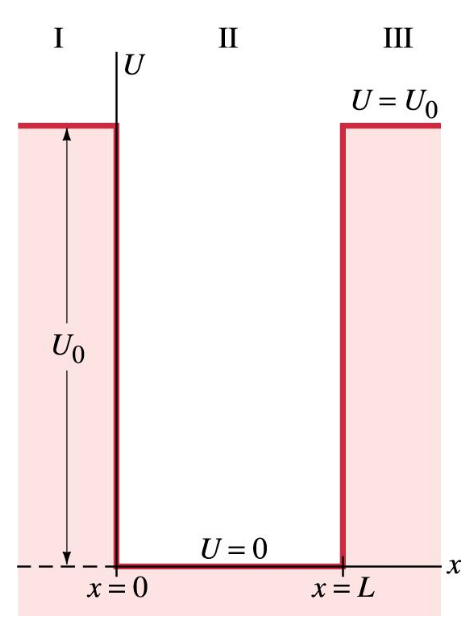
\includegraphics[width=0.4\columnwidth]{images/potentialwell.png}
    \label{fig:my_image}
\end{figure}
Potential energy to the left and right of the potential well is finite:
\begin{equation*}
 V = \,
\left\{
  \begin{array}{l}
    0 \qquad 0 \le x \le L \\
    U_{0}\qquad 0 < x\,\text{and} > L\\
  \end{array}
\right.
\end{equation*}
Three Areas \rom{1},\rom{2} and \rom{3}, in \rom{2} \((0 \le x \le L)\) particel is free:
\begin{equation*}
    \psi_{\rom{2}}(x) = A_{\rom{2}} \cdot \sin(k\cdot x - \varphi) \quad \text{with:}\quad k = \frac{2\pi}{\lambda} = \sqrt{\frac{2\cdot m}{\hbar^2}\cdot E}
\end{equation*}
but without the limitation \(\psi(0) = \psi(L) = 0\).
\textbf{For \(E \le U_0\) the following applies in areas \rom{1} and \rom{3}}:
\begin{equation*}
    \psi(x) = A_1 \cdot e^{b\cdot x} + A_2 \cdot e^{b\cdot x} \quad \text{with:}\quad b = \sqrt{\frac{2\cdot m}{\hbar^2}\cdot(U_0 - E)}
\end{equation*}
\begin{equation*}
    \psi_{\rom{1}} = A_{\rom{1}} \cdot e^{b\cdot x} \quad  \text{with} \quad A_{\rom{3}} \cdot e^{-b\cdot x} 
\end{equation*}
Exponential drop to the left and right. On the walls, both the wave function and its derivative must be continuous:
\begin{equation*}
    \left.\psi_{\rom{1},\rom{3}}\right|_{x = 0,L} =
    \left.\psi_{\rom{2}}\right|_{x = 0,L}
    \quad \text{and} \quad
    \left.\frac{d\psi_{\rom{1},\rom{3}}}{dx}\right|_{x = 0,L} =
    \left.\frac{d\psi_{\rom{2}}}{dx}\right|_{x = 0,L}
\end{equation*}

\textbf{If \(E > U_0\) the solution in the areas \rom{1} and \rom{3} is also a harmonic wave:}
\[
E - U_0 = \frac{p^2}{2m} = \frac{h^2}{2m\lambda}
\]
\begin{equation*}
    \psi(x) = A\cdot \sin(k\cdot x-\varphi)\quad\text{with:}\quad k= \frac{2\pi}{\lambda} = \sqrt{\frac{2\cdot m}{\hbar^2}\cdot(E-U_0)}
\end{equation*}
The wavelength in these areas is greater than in area \rom{2}.
\subsubsection{Potential step \(E > U_0\)}
A part of the incident wave is reflected or transmitted at each transition. We know:
\begin{equation*}
    A_r = \frac{k_1 - k_2}{k_1 + k_2}\cdot A_{ein}, \quad A_t = \frac{2\cdot k_1}{k_1 + k_2} \cdot A_{ein}
\end{equation*}
So there is a certain probability that a particel will be reflected
\begin{equation*}
    R = \frac{(k_1 -k_2)^2}{(k_1 + k_2)^2}
\end{equation*}
We find the wave numbers
\begin{equation*}
    k = \frac{2\pi}{\lambda} = \sqrt{\frac{2 \cdot m}{\hbar^2}\cdot (E-U_0)}
\end{equation*}
\subsection{Quantum Tunnelling}
\begin{figure}[h]
    \centering
    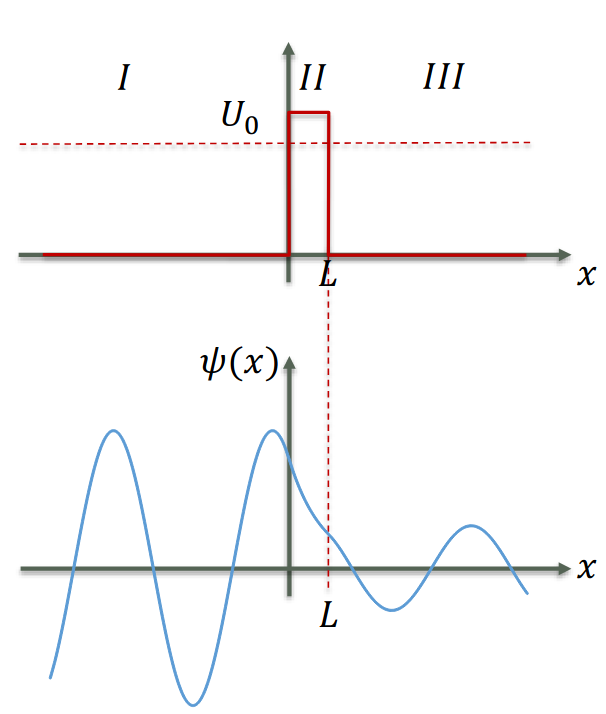
\includegraphics[width=0.4\columnwidth]{images/tunnel.png}
    \label{fig:tunnel}
\end{figure}
Exponential decrease with barrier with. \textbf{Probability of tunneling:}
\begin{equation*}
    T \approx e^{-2\cdot b\cdot L} \quad\text{with:}\quad b = \sqrt{\frac{2\cdot m}{\hbar^2}\cdot (U_0 - E)}
\end{equation*}
Examples: Radiactive \(\alpha\) deacy, electron microscope
\subsection{Quantum harmonic oscillator}
\begin{figure}[h]
    \centering
    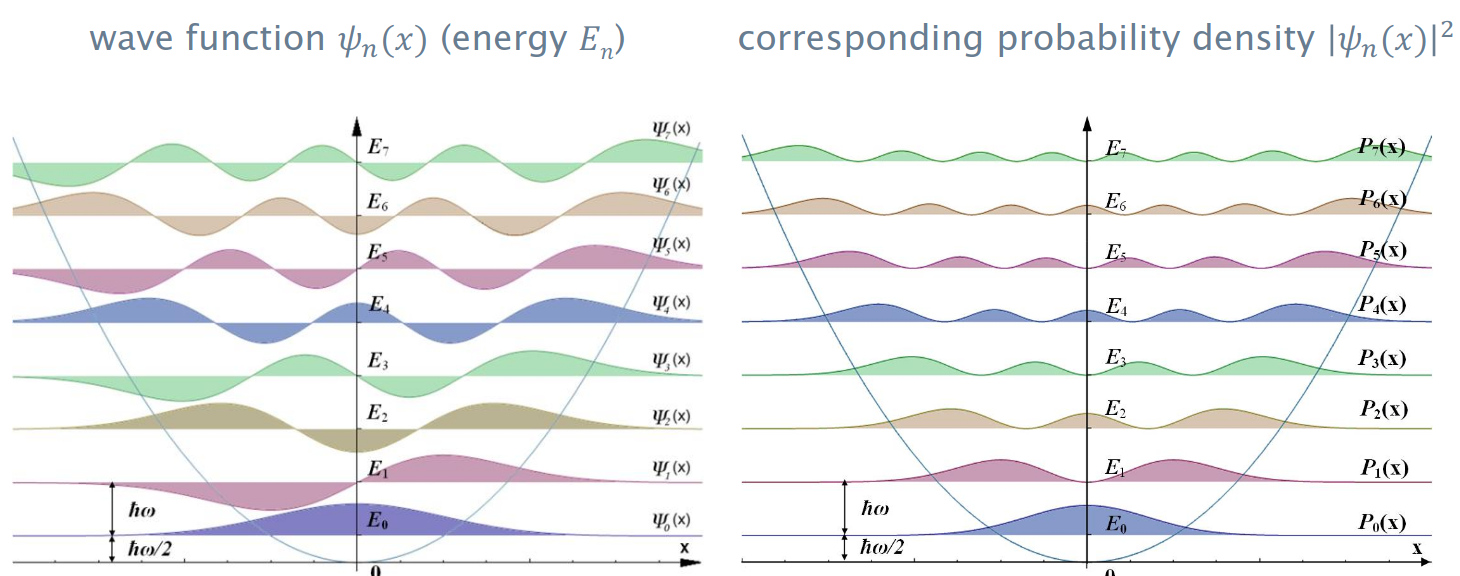
\includegraphics[width=\columnwidth]{images/harmoicoszillator.png}
    \label{fig:harmoszi}
\end{figure}
Complex math to get to \(\psi\).
Energy:
\begin{equation*}
    E_n = \hbar \cdot \omega\cdot (n + \frac{1}{2})\quad \text{with:}\quad n \in \mathbb{N}_0
\end{equation*}
Quantized, Equally spaced, Zero-point energy \(E_0 = \frac{1}{2}\hbar\omega\)
\begin{equation*}
    V(x) = \frac{1}{2}\cdot k \cdot x^2 = \frac{1}{2}\cdot m\cdot \omega^2 \cdot x^2
\end{equation*}
\section{Atoms}
For hydrogen atom, the potential (potential energy) is given by the spherically symmetric Coulomb potential:
\begin{equation*}
    V(r) = - \frac{1}{4\cdot \pi \cdot \epsilon_0}\cdot\frac{e^2}{r}
\end{equation*}
\(\epsilon_0\) permittivity of vacuum, \(e\) elemntary charge.

\begin{equation*}
    E_n = -\frac{m\cdot e^4}{8 \cdot \epsilon_0^2 \cdot h^2}\cdot\frac{1}{n^2}
    = -\frac{E_1}{n^2} = -\frac{13.6 \,\text{eV}}{n^2} 
\end{equation*}
with \(n = 1,2,3,\dots\).
Here \(n\) is the principal quantum number and defines the energy \(E_n\) belonging to the wave function \(\psi_{n.l,m}(r,\theta,\varphi)\)
\[
\psi_{1,0,0}(r,\theta,\varphi) = \frac{1}{\sqrt{\pi r_0^3}}\cdot e^{-\frac{r}{r_0}}
\]
\subsection{Quantum numbers}
\begin{itemize}
    \item \(n\) -- Principal quantum number (shell)
    \item \(l\) -- Azimuthal quantum number
    \item \(m_l\) -- Magentic quantum number
    \item \(m_s\) -- Spin quantum number (\(\pm \frac{1}{2}\)for electrons)
\end{itemize}

\subsection{Pauli exclusion principle}
Electrons as fermions (half integer spin)\(\rightarrow\) two electrons (inan atom) cannot be in the same quantum state.

\subsection{Molecules}
Two hydrogen atoms approach each other:
\begin{itemize}
    \item Parallel spins: \(S = \frac{1}{2} + \frac{1}{2} = 1\), Pauli principle \(\rightarrow\) No bond
    \item Antiparallel spins: \(S = \frac{1}{2} - \frac{1}{2} = 0\), Electron more likely inbetween nuclei \(\rightarrow\) attraction of the positiv nuclei to the electron cloud \(\rightarrow\) Covalent bond.
\end{itemize}
\subsection{Molecular (Organic) Semiconductors}
\begin{figure}[h]
    \centering
    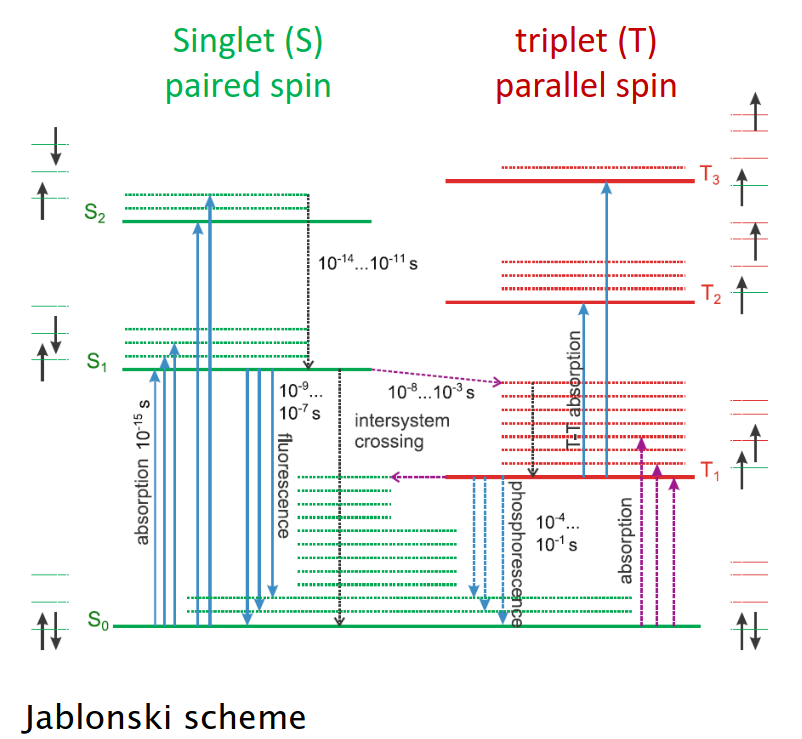
\includegraphics[width=\columnwidth]{images/jablonski.png}
    \label{fig:jablonski}
\end{figure}
\begin{itemize}
    \item Blue arrows: spin allowed transitions \(\rightarrow\) likely
    \item Dashed green and red lines: vibrational states
    \item Emission of photons mainly due to:
    \subitem Fluorescence (fast)
    \subitem Phosphorescence (slow)
\end{itemize}

\subsection{Electron Theory of Metals}
Electron are trapped in the metal like a potential well.
Within the metal(potential well) the potential energy is zero.
There are high potential walls at the metal edges.
Only a few electrons escape from the metal at room temperature(infinite potential well).
At higher temperatures electrons escape (thermal emmissions)(finite potential well).
In the potential well with macroscopic size, electrons can move freely.
Energy is quantized, distance between energy levels is very small (\(L\) very large).
\begin{equation*}
    E_n = n^2 \cdot \frac{h^2}{8 \cdot m \cdot L^2} = n^2 \cdot \frac{\hbar^2 \pi^2}{2\cdot m \cdot L^2} = n^2 \cdot E_1
\end{equation*}
Large number of states so close together that they seem to from a continuum.
Calculation of physical properties of conduction electrons by statistical meth ods.
Density of state \(g(E)\):
\begin{equation*}
    g(E) = \frac{8\sqrt{2}\pi m^{\frac{3}{2}}}{h^3}\sqrt{E}
\end{equation*}
\(g(E)\,dE\) indicates the number of states per volume unit that have energies between \(E\) and \(E + dE\).
\begin{figure}[h]
    \centering
    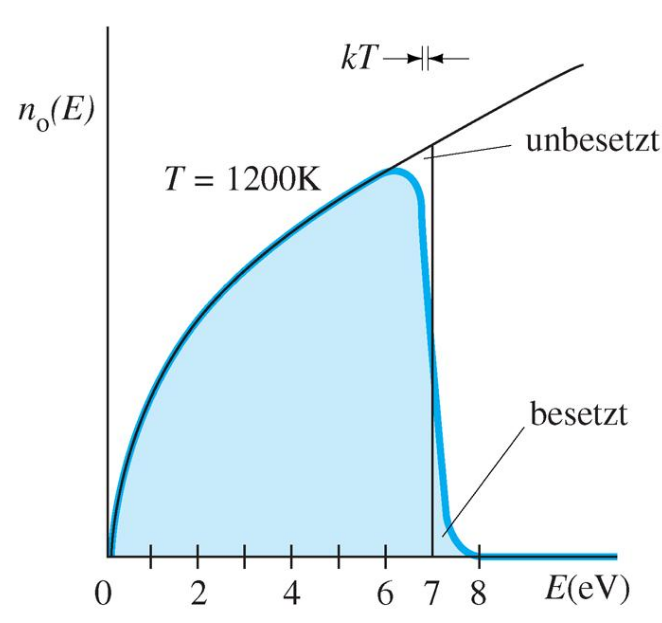
\includegraphics[width=0.8\columnwidth]{images/metals.png}
    \caption{Vertical black line: Fermi-Level}
    \label{fig:metals}
\end{figure}
Energy at Fermi level is called Fermi energy.
To determine the Fermi energy, we integrate from \(E = 0\) to \(E = E_F\):
\[
\frac{N}{V} = \int_{0}^{E_F}g(E)\, dE
\]
solving for \(E_F\):
\[
E_f = \frac{h^2}{8m}\left(\frac{3}{\pi}\frac{N}{V}\right)^{\frac{2}{3}}
\]
Mean energy:
\[
\overline{E} = \frac{3}{5}E_F
\]

In case of electron gas, a quantum mechanical system that is subject to the pauli principle, the occupation of a given state with that of the energy \(E\) is given by the Fermi-Dirac distribution:
\[
f(E) = \frac{1}{e^{(E-E_F)/kT} + 1}
\]
Occupation density:
\[
n_0(E) = g(E)\cdot f(E)
\]
\subsubsection{Calulations}
To approx \(N\)(Number of states) over a given range \(E + \Delta E\) and Volume \(V\). For exact values integrate \(g(E)\). For approximation take value in the middel(\(g(E + \frac{1}{2}\Delta E)\))
\begin{equation*}
    N \approx g(E + \frac{1}{2}\Delta E) \cdot V \cdot \Delta E
\end{equation*}
\subsection{Energy bands}
\begin{figure}[h]
    \centering
    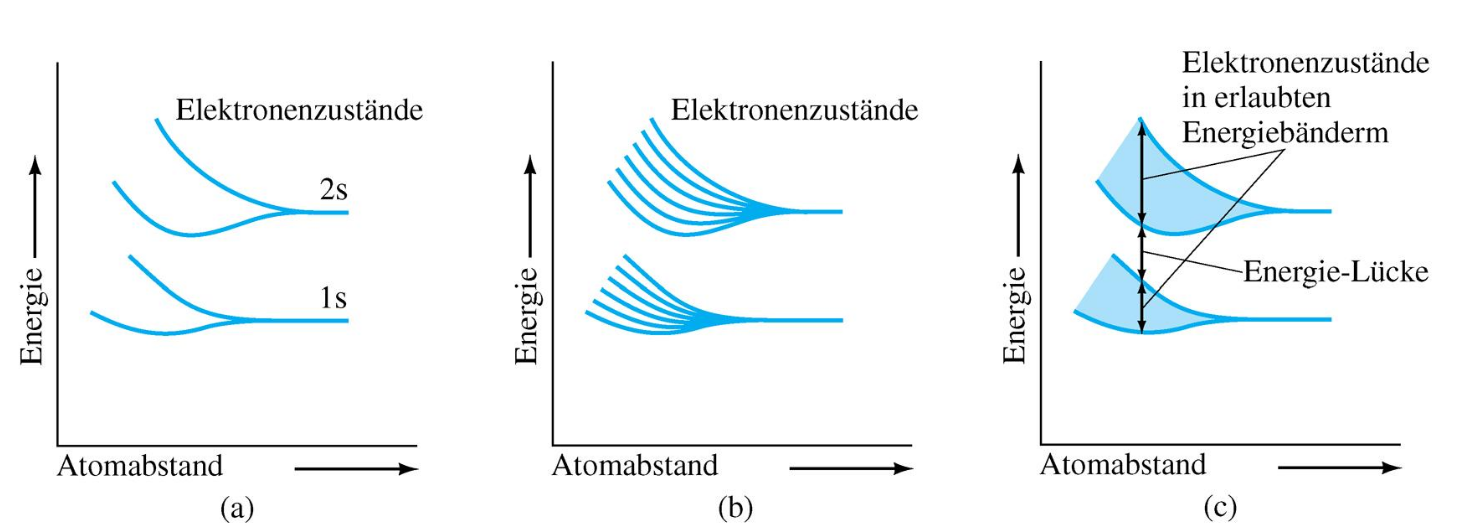
\includegraphics[width=\columnwidth]{images/bandmodel.png}
    \label{fig:bandmodel}
\end{figure}
The electrical conductivity of a crystal depends on how the highest energyband filled with electrons is filled: empty, partially filled, completely filled.
\begin{itemize}
    \item \textbf{Conductor:} The highest energy band occupied by electrons is only partially filled.
    \item \textbf{Insulator:} The highest band filled with electrons, the valence band, is completly filled.
    \item \textbf{Semiconductor:}The bands of a pure semiconductor are similar to those of an insulator, but the unfilled conduction band is seperated from the valence band by a much smaller band gap \(E_g\approx 1 \text{eV}\)
\end{itemize}
\subsubsection{Semiconductors}
Due to the small band gap, at room temperature, some electrons can absorb enough thermal energy to reach the conduction band, so that a very small current flows when voltage is applied.
The higher the temperature the more electrons overcome the band gap.
\begin{figure}[h]
    \centering
    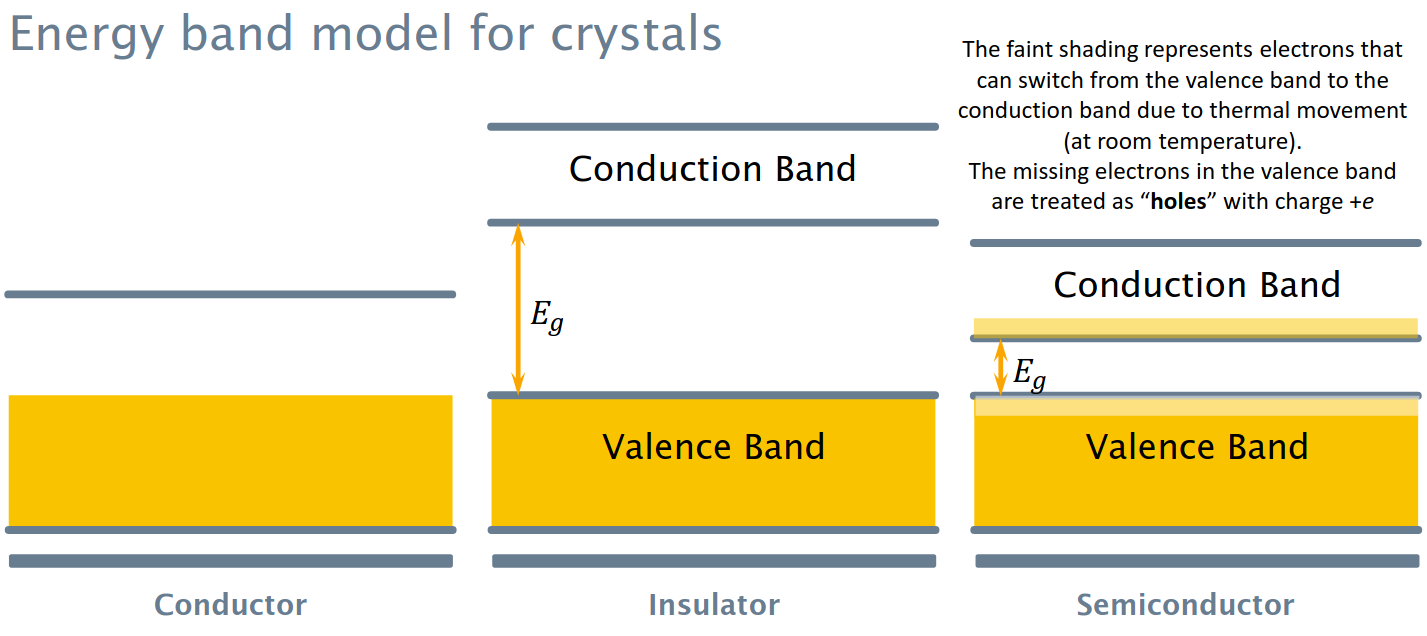
\includegraphics[width=\columnwidth]{images/bandmodel2.png}
    \label{fig:bandmodel2}
\end{figure}

\textbf{n-doping:} Additional electron added by donors(e.g. P in Si) goes in conduction band, More electrons \(\rightarrow\) Fermi level shifts to CB

\textbf{p-doping:} Missing electron acceptors(e.g. B in Si) creates hole, More holes \(\rightarrow\) Fermi level shifts to VB

\section{Absorption and emission}
\textbf{Black Body:}
\begin{itemize}
    \item Absorption = \(100\%\) for all wavelengths
    \item Emission:
    \subitem Thermal radiation
    \subitem Temperature dependent
    \subitem Planck's law 
\end{itemize}


 \subsection{Conductivity}
 Electrical resistance:
 \[
 R = \frac{U}{I}= \rho\frac{l}{A} = \frac{1}{\sigma}\frac{l}{A}
 \]
 \(\rho\): Resistivity, Ohm com
 
 \(\sigma\): Conductivity, Siemens/cm
 \[
 I = e \cdot n \cdot v \cdot A
 \]
 \(e\): elementary charge

 \(n\): electron density in \(\text{cm}^3\),\(v\) velocity
\[
\text{Mobility}\, \mu = -\frac{v}{E}
\]
\[
\sigma = e \cdot n \cdot \mu
\]
In a semiconductor, we have holes with concentration \(p\) as well, thus:
\[
\sigma = e \cdot (n\cdot \mu_n + p \cdot \mu_p)
\]
\[
\mu = \frac{e}{m^*} \cdot \tau
\]
\(\tau\): time between scattering events

\(m^*\): effective electron mass


\section{Photonic Crystals}
Photonic band-gap (PBG) materials or photonic crystals (PC) are materials
with a periodic dielectric profile,
which can prevent light of certain frequencies or wavelengths
from propagating in one, two or any number of polarisation directions
within the materials.
This range of frequencies is analogous to an electronic band-gap.
Thus, it is often called a photonic band-gap.

Some wavelengths cant propagate though crystals: \(\lambda\approx 2 a\)

\begin{itemize}
    \item Electrons are waves (quantum mechanics)
    \item Waves in a periodic medium can propagate without scatterning: Bloch's Theorem
    \item The foundations do not depend on the specific wave equation.(Hold for magnetic waves as well)
\end{itemize}

\subsection{Periodic Hermitian Eigen-problems in 1D}
\begin{itemize}
    \item Start with a uniform(1D) medium
    \item Treat it as \textit{artificially} periodic
    \item Bands are folded by \(2\pi/a\) equivalence
    \item Add a small real preiodicity \(\epsilon_2 = \epsilon_1 + \Delta\epsilon\)
    \item Splitting of degeneracy: state concentrated in higher index \(\epsilon_2\) has lower frequency \(\omega\)\((\omega = \frac{c}{\sqrt{\epsilon_1}}k = \frac{c}{n}k)\)
\end{itemize}
\begin{figure}[h]
    \centering
    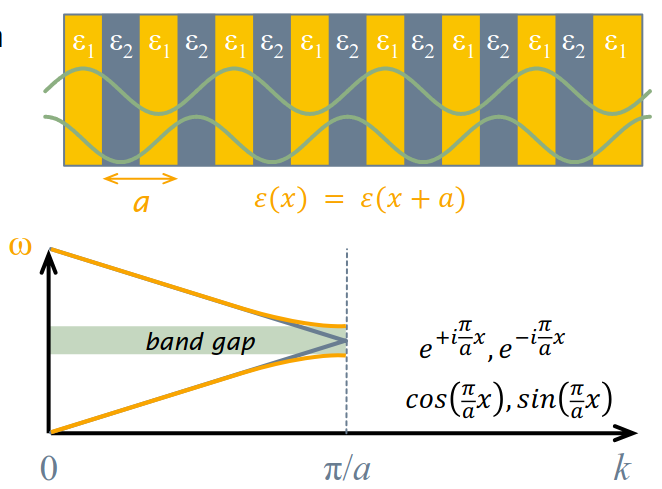
\includegraphics[width=\columnwidth]{images/eigenproblem.png}
    \label{fig:eigenmodel}
\end{figure}

	\section{Scaling laws}


Metal organic framework(MOF): porus materials. Able to store substance (e.g. Water) at low temperature and release when heated.

Void volume (porosity) is defined as
\[
\epsilon = \frac{V_pores}{V_materials}
\]
\begin{itemize}
    \item Micropores (<2nm)
    \item Mesopores (2-50nm)
    \item Macropores (>50nm)
\end{itemize}
\subsection{Surface Tension and surface energy}
Water runner on water, leg sinks \(\rightarrow\) Energy is stored in surface energy:
\[
E_s = \gamma \cdot A
\]
\(\gamma\): specific surface energy/surface tension \(\text{J/m}^2\) or \(\text{N/m}^2\) 

The surface tension tries to keep the surface of a fluid as small as possibel \(\rightarrow\) Drops of liquid are spherical.
\[
V(r) = -\frac{A}{r} +B \cdot r^{-n}
\]
\[
K_s = \frac{d^2V}{dr^2} \qquad \frac{K_s}{a_a} \sim \frac{1}{a_0^{-4}}
\]%Todo Checken 
\section{Condensed matter}
Type of bonds:
\begin{itemize}
    \item \textbf{Ionic Bond:} Metal atom donates electron to nonmetal atom
    \item \textbf{Covalnet Bond:} Two nonmetalatoms share electrons
    \item \textbf{Metallic Bond:} Electrons move freely between atoms
\end{itemize}
\textbf{Van der Waals force:} weak dipole dipole charge interaction between molecules(e.g. water, polymers, proteins).

\subsection{Surface of solid}
\begin{figure}[h]
    \centering
    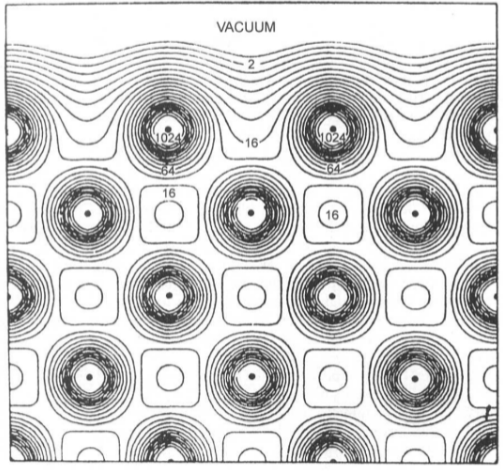
\includegraphics[width=0.7\columnwidth]{images/surface.png}
    \label{fig:surface}
\end{figure}
\begin{itemize}
    \item Surface represent typcalliy \(15\)\r{A}
    \item At the surface, positiv periodic potential due to ions cores terminates
    \item Electrons will screen out at the surface resulting in  increased electron density
    \item At the surface, charge density is smeared out and less periodic compared to the interior ion cores(potential decrease)
    \item This smoothing of the surface charge is the compromise electrons strike when they lower both their potential and kinetic energies
    \item Band bending or new states happen at the surface
\end{itemize}
\begin{figure}[h]
    \centering
    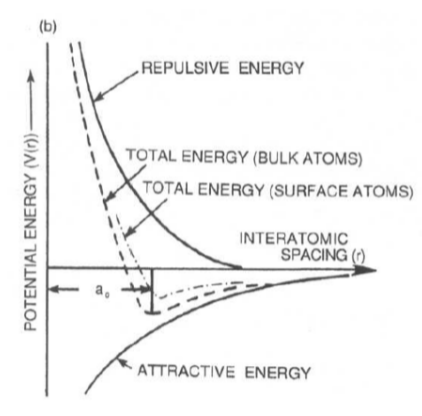
\includegraphics[width=\columnwidth]{images/atombond.png}
    \label{fig:atombond}
\end{figure}
\subsubsection{Adsorption on solid surface}
Rate at which physisorption molecules become chemisorbed:
\[
k = v_0 \exp\left(-\frac{E_a}{kT}\right)
\]
\begin{figure}[h]
    \centering
    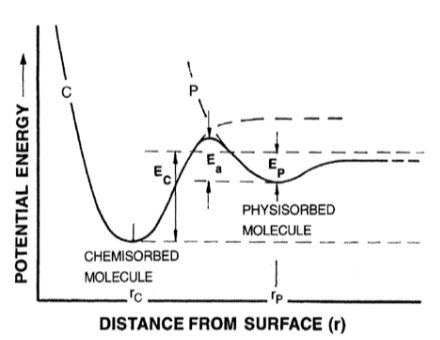
\includegraphics[width=0.7\columnwidth]{images/surfacedistance.png}
    \label{fig:surfdist}
\end{figure}
\textbf{Surface adsorption: }Impinging atoms and molecules enter and interact within the transition region between gas phase \& Surface

Two kinds:
\begin{itemize}
    \item \textbf{Physisorption:} Van der waals force bond particel to the Surface
    \item \textbf{Chemisorption:} Particel changes identity through ionic or covalnet bonding with subtrate atoms
\end{itemize}

\subsection{Capillary theory of nucleation}
\begin{figure}[h]
    \centering
    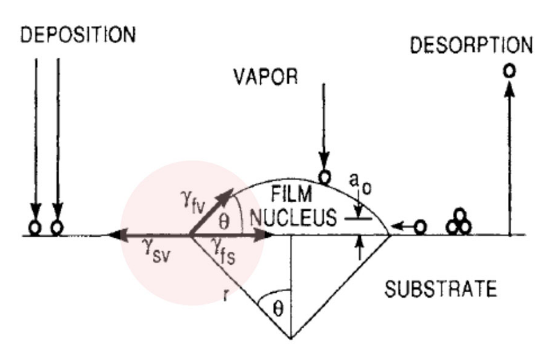
\includegraphics[width=0.7\columnwidth]{images/nucleation.png}
    \label{fig:nucleation}
\end{figure}
Film forming atoms or molecules in the vapor phase impinge on the substrate creating nuclei of mean dimension \(r\)

Spherical cap:
\[
a_1 = 2\Pi\left[1 -  \cos(\theta)\right]
\]
\[
a_2 = \Pi\cdot\sin^2(\theta)
\]
\[
a_3 = \frac{\Pi}{3}\left[2 - 3\cos(\theta) + \cos^3(\theta)\right]
\]
Free-energy change:
\[
\Delta G = a_3 r^3 \Delta G_v + a_1 r^2 \gamma_{fv} + a_2 r^2 \gamma_{fs} - a_2 r^2 \gamma_{sv}
\]
Mechanical equilibrium among horizontal components(Youngs equation):
\[
\gamma_{sv} = \gamma_{fs} + \gamma_{fv} \cos(\theta)\quad\text{or}\quad \cos(\theta) = (\gamma_{sv} -\gamma_{fs})/\gamma_{fv}
\]
Critical nucleus size \(r = r^*\):
\[
r^* = \frac{-2(a_1 \gamma_{fv}+a_2 \gamma_{fs} - a_2 \gamma_{sv})}{3 a_3 \Delta G_v}
\]
\subsection{Film growth modes}
Island growth:
\[
 \gamma_{sv} < \gamma_{fs} + \gamma_{fv}
\]
Layer growth:
\[
\gamma_{sv} \ge \gamma_{fs} + \gamma_{fv}
\]
\begin{figure}[!ht]
    \centering
    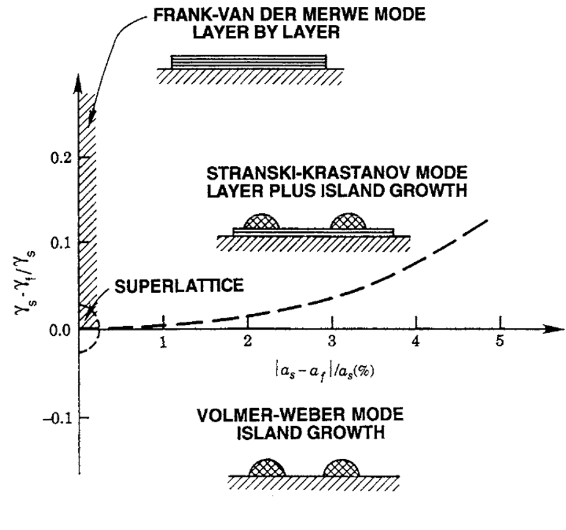
\includegraphics[width=\columnwidth]{images/layergrowth.png}
    \label{fig:layergrowth}
\end{figure}
\begin{figure}[!ht]
    \centering
    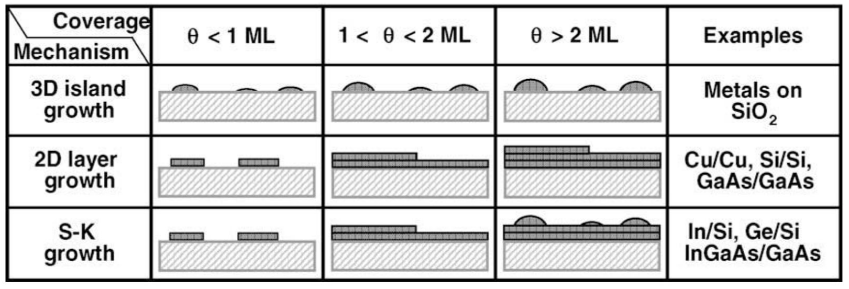
\includegraphics[width=\columnwidth]{images/growthmode2.png}
    \label{fig:growthmode2}
\end{figure}

\subsection{Dewetting}
\begin{figure}[h]
    \centering
    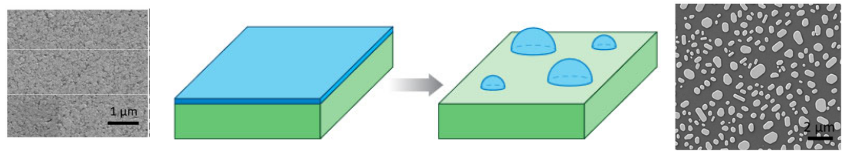
\includegraphics[width=\columnwidth]{images/dewetting.png}
    \label{fig:dewetting}
\end{figure}
During solid-state dewetting, thin films dewet to form isolated islands. This occures while the material remains in the solid state.
\begin{itemize}
    \item Thin films dewet or agglomerate to form arrays of islands when heated.
    \item This can happen when a films melting temperatures so that dewetting (agglomeration) occures while the film remains in the solid state.
    \item Driving force: minimization of the total energy of the free surfaces of the film and substrate, and of the film-substrate interface.
\end{itemize}

\subsection{Calculation of Surface energy}
OWRK-model:
\[
\sigma_{SL} = \sigma_{S} + \sigma_{L} - 2\sqrt{\sigma_S^d\sigma_L^d} - 2\sqrt{\sigma_S^p\sigma_L^p}
\]
With Youngs equation get linear equation \(y = mx + c\):
\[
\underbrace{\frac{\sigma_L (1+\cos(\Theta))}{2\sqrt{\sigma_L^d}}}_{y} 
= 
\underbrace{\sqrt{\sigma_S^p}}_{m}
\cdot
\underbrace{\frac{\sigma_L^p}{\sigma_L^d}}_{x} 
+ 
\underbrace{\sqrt{\sigma_s^d}}_{c}
\]
\(\sigma\) sometimes given as \(\gamma\)

\(S\): Solid

\(V\): Vapor

\(L\): Liquid

\[
\sigma_{tot} = \frac{d_{21}\sigma_{21} + d_{22}\sigma_{22}}{d_{tot}} \quad \sigma = -\left(\frac{E}{1-V}\right)\left(\alpha_f- \alpha_s\right)\Delta T
\]
\section{Stress in thin film}
\

Film exerts bending moment on substrate plate which leads to curvature \((K = 1/R)\)
\begin{figure}[!ht]
    \centering
    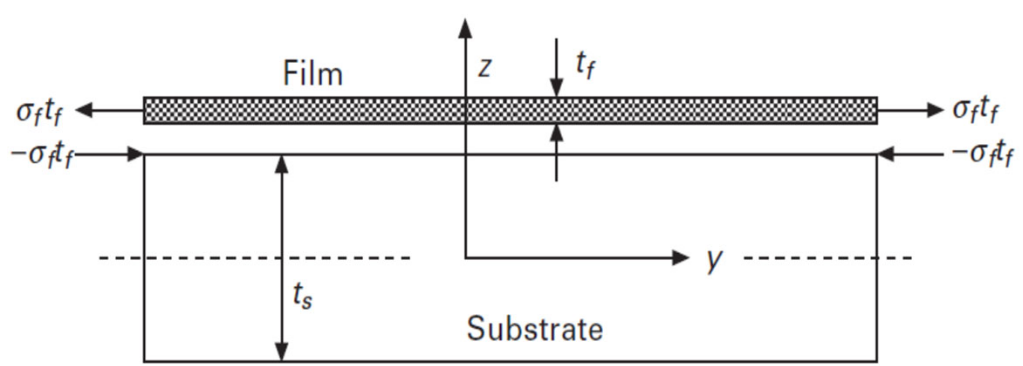
\includegraphics[width=\columnwidth]{images/stoney.png}
    \label{fig:stoney}
\end{figure}

\textbf{Stoney equation:}
\[
\sigma_f = \left(\frac{E_s}{1-v_s}\right)\frac{t^2_s}{6 t_f}\Delta \kappa
\]
Term \(\left(\frac{E_s}{1-v_s}\right)\) is called biaxial elastic modulus.

\(\kappa\): Curvature

Stoney equation is independent of film properties. Appliccable for thin film on a much thicker substrate.

\textbf{Methods for residual stress measurments:}
\begin{itemize}
    \item \textbf{Mechanical methods:} Substrate curvature vie laser deflection, bending of Focused Ion Beam(FIB) bi-metal beam
    \item XRD, Raman specrtoscopy 
\end{itemize}

Method comperison: Spatial (lateral \& depth), and spectral resolution

Stress types:
\begin{itemize}
    \item \textbf{Thermal:} Mismatch of thermal expansion coefficients
    \item \textbf{Intrinsic:} During Film growth
    \item \textbf{epitaxial(Misfit):} Lattice mismatch with substrate
\end{itemize}

\begin{figure}[h]
    \centering
    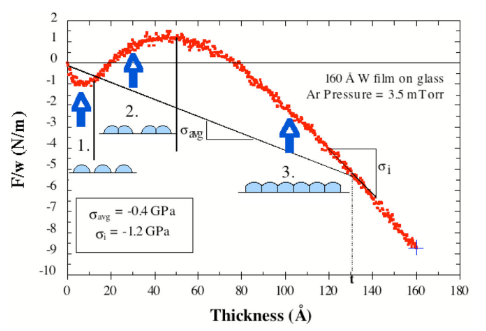
\includegraphics[width=\columnwidth]{images/insitu.png}
    \label{fig:insitu}
\end{figure}

\textbf{The stress dilemma:} intrinsic stress relaxes at high deposition T, thermal increases

\subsection{Adhesion of thin films}

Stress intensity at crack tip:
\[
K = 0.7 \sigma\sqrt{h}
\]

Energy release rate if interface crack propagates:
\[
G = 0.5 \frac{1-v^2}{E}\sigma^2 h
\]

\textbf{Strategies against bad film adhesion - glue layers:} It is common to first deposit a fed hundered angstroms of an intermediate oxygen-active metal to serve as the \textit{glue} between the film and substrate.

Scratch Testing:
\begin{itemize}
    \item Draw diamond tip across surface with increasing normal load until a critical event occures
    \item Film will debond(form buckle) or fracture(form through thickness cracks)
\end{itemize}

\subsection{Hard Coatings}
Hard materials: mixed bonds(covalent + metallic + ionic)
Three groups are distinguished based on chemical bonding:
\begin{itemize}
    \item \textbf{metallic hard materials}(covalent + metallic)
    \subitem +: adhesion, toughness ductility, high elastic modulus
    \item \textbf{ionic hard materials}(covalent + ionic)
    \subitem +: hardness, thermodynamic stability, \\chemical inertness
    \subitem -: very brittle
    \item \textbf{covalent hard materials}(covalent + ionic)
    \subitem +: hardest materials(Diamond), strength, high temperature strength, low thermal expension coefficant
    \subitem -: not adapted to metallic substrate at HT
\end{itemize}

The \textbf{intrinsic hardness }related to:
\begin{itemize}
    \item high binding energy (bond strength)
    \item short interatomic distance (small bond lenght)
    \item high degree of directional covalent bonds(ionicity and metallicity decrease hardness)
    \item high number of valence electrons per atom
    \item high number of bonds per unit volume
\end{itemize}

\section{Optical coatings}
\begin{figure}[h]
    \centering
    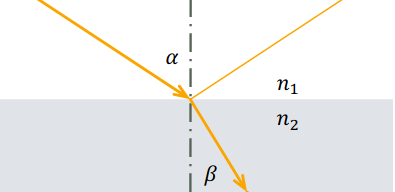
\includegraphics[width=0.7\columnwidth]{images/fresnel.png}
    \label{fig:fresnel}
\end{figure}
Fresnel refraction:
\[
n_1 \sin(\alpha) = n_2 \sin(\beta)
\]
Reflected power/Incident power:
\[
R = \left(\frac{n_2-n_1}{n_1 + n_2}\right)^2
\]
Transmitted power/Incident power:
\[
T = \frac{4n_1n_2}{\left(n_1+n_2\right)^2}
\]
with \(R + T = 1\)

\subsection{Interference}
\begin{figure}[h]
    \centering
    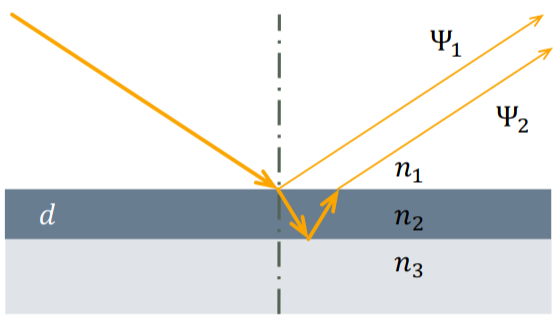
\includegraphics[width=0.7\columnwidth]{images/ThimFilmInterference.png}
    \label{fig:fresnel}
\end{figure}
\(n_2 = \sqrt{n_1 \cdot n_3}\) for diminating reflection (Equal amplitude reflection \(\psi_1 = \psi_2\))

\textbf{Constructive Interference:} Superposition of two waves which are in phase

\textbf{Destructive Interference:} Superposition of two waves with a phase shift of \(\pi\)

Thin film interference \(n_1 = 1 \text{ Air} < n_2, n_3\)

Case 1:\(n_2 < n_3\)
\begin{itemize}
    \item Phase jumps of \(\pi\) for both waves
    \item Destructive interference for \(d \cdot n_2 = \lambda_0/4\)
\end{itemize}
Case 2:\(n_2 > n_3\)
\begin{itemize}
    \item Phase jump upper interface, no phase jumps at lower interface
    \item Constructive interference for \(d\cdot n_2 = \lambda_0/4\)
\end{itemize}

\section{Ineraction of light with nano and microparticels}
\textbf{Dielectric}
\begin{itemize}
    \item Bound electrons \(\rightarrow\) Lorentz Model for dielectric function
    \item Spring effect between electron-ion
    \item Dampening due to collisions
    \item Electric field
\end{itemize}

Lorentz dielectric function:
\[
\epsilon(\omega) = 1 + \frac{\omega^2_p}{(\omega_0^2-\omega^2)+i\gamma \omega}
\]
\textbf{Metal}
\begin{itemize}
    \item Free electrons \(\rightarrow\) Drude Model for dielectric function
    \item Spring effect between electron-ion
    \item Dampening due to collisions
    \item Electric field
\end{itemize}

Drude dielectric function:
\[
\epsilon(\omega) = 1 + \frac{\omega^2_p}{i\gamma \omega-\omega^2}
\]
with \(\omega^2_p = \frac{Nq^2}{m_e\epsilon_0}\),\(\gamma = \frac{1}{\tau}\) and \(\tau = \text{time between collisions}\)

\[
R = \frac{\left(n-1\right)^2 + k^2}{\left(n+1\right)^2 + k^2}
\]
\[
E(x,t) = E_0 e^{i\left(kx - \omega t\right)}
\]
\[
k = \frac{2\pi}{\lambda} = \frac{\omega}{c} = \frac{n\omega}{c}
\]
If ignore dampening: \(\rightarrow \epsilon(\omega) = 1 + \frac{\omega^2_p}{\omega}\)
\[
N(\omega) = \sqrt{\epsilon(\omega)} = \sqrt{1 + \frac{\omega^2_p}{\omega}}
\]
\[
\omega < \omega_p \rightarrow n=0,\,k\neq0 \rightarrow R = 1
\]
\[
\omega > \omega_p \rightarrow n=1,\,k\neq0 \rightarrow R = 0
\]
\subsection{Scattering}
 \textbf{Rayleigh Scattering (elastic):}
 \begin{itemize}
    \item Interaction between light (photon) and air (\(\text{N}_2\) symmetrical molecule)\(\lambda \ll d\)
    \item Elastic coupling varying E field and dipole
    \item (\(\Theta\) parameter): Scattering at right angles is half the forward/backward intensity
 \end{itemize}
 \textbf{Mie Scattering:}
 \begin{itemize}
    \item For \(\lambda/10 < r < \lambda\)
    \item n case of visible light 400-780nm, particles between 50-500 nm
    \item Amount of scattered light \(\text{Q} \approx \text{extinction coefficient}\approx c+\cos(r/\lambda)e^{-kr/\lambda}\)
 \end{itemize}

	% \input{Sections/14-GenerativeAI.tex}

\end{document}
